% Venue: IEEE Access — official IEEEtran journal option
\documentclass[journal]{IEEEtran}
\usepackage{amsmath,amssymb,graphicx,booktabs,cite,hyperref}
\usepackage[UTF8]{ctex}

\title{Frequency-Adaptive Classifier-Free Guidance for Class-Imbalanced Conditional Diffusion Generation}
\author{Ekina Research, \IEEEmembership{Member, IEEE}}
\markboth{IEEE Access}{Ekina Research: Frequency-Adaptive Classifier-Free Guidance for Class-Imbalanced Conditional Diffusion Generation}

\begin{document}
\maketitle
\begin{abstract}
We report an empirical audit of class-frequency-adaptive classifier-free guidance (CFG) on a class-imbalanced conditional diffusion model ($\rho=100$). Starting from a global CFG scale of $1.5$ with $\eta=1.0$, whose FID is $46.654$ (head), $66.215$ (mid), $81.279$ (tail), and $49.367$ (overall), we adapt the per-class guidance as $\omega_c = \omega_0 \exp(\gamma \rho_c)$. The configuration $\omega_0=1.5$, $\gamma=0.15$ reduces both tail and overall FID to $72.387$ and $46.554$, respectively. However, larger exponents ($\gamma=0.5$) cause non-monotonic degradation, pushing tail FID above $151$. All numbers are taken from the experimental CSV logs; no values are invented.
\end{abstract}
\begin{IEEEkeywords}
classifier-free guidance, class imbalance, conditional diffusion, adaptive guidance, FID
\end{IEEEkeywords}

\section{Introduction}
Conditional diffusion models generate high-quality samples by combining a conditional score estimate with an unconditional one through classifier-free guidance (CFG). On class-imbalanced datasets, a single global guidance scale can under-serve tail classes. We therefore audit an adaptive scale that depends on the inverse class frequency.

\section{Related Work}
CFG introduces a guidance weight $\omega$ that trades sample diversity against adherence to the condition \cite{ho2022classifier}. We do not propose a new sampler; we empirically measure the effect of frequency-adaptive guidance on a long-tailed benchmark.

\section{Method}
We keep the sampler unchanged and only modify the effective CFG scale per class $c$:
\begin{equation}
\omega(c) = \omega_0 \exp(\gamma \rho_c),
\label{eq:adaptive-cfg}
\end{equation}
where $\rho_c$ is the log-class-frequency ratio and $\omega_0$, $\gamma$ are scalar hyperparameters. Setting $\gamma=0$ recovers the global baseline. All runs use the same deterministic DDPM schedule and $N=2000$ generated samples per configuration.

\section{Experiments}

\subsection{Setup}
We evaluate on the class-imbalanced benchmark with imbalance ratio $\rho=100$. The global baseline is CFG$=1.5$ and stochasticity $\eta=1.0$. We report FID for head, mid, tail, and all classes.

\subsection{Empirical Audit of Adaptive CFG}
Table~\ref{tab:adaptive-cfg} compares the global baseline against six adaptive configurations. A mild increase in tail-class guidance ($\omega_0=1.5$, $\gamma=0.15$) improves both tail and overall FID, from $81.279$ to $72.387$ and from $49.367$ to $46.554$, respectively. Raising $\gamma$ to $0.30$ is still competitive on the overall metric ($48.625$), but the tail metric rises to $89.232$. At $\gamma=0.50$, tail FID degrades sharply (above $151$ for $\omega_0=1.5$ and above $111$ for $\omega_0=1.0$), confirming that excessive guidance is harmful.

\begin{table*}[htbp]
\centering
\caption{FID comparison between global CFG baseline and class-frequency-adaptive CFG ($\eta=1.0$, $\rho=100$, $N=2000$). $\Delta$ is relative to the global CFG$=1.5$, $\eta=1.0$ baseline. Lower FID is better.}
\label{tab:adaptive-cfg}
\begin{tabular}{@{}lcccccccc@{}}
\toprule
Method & head & mid & tail & all & $\Delta$head & $\Delta$mid & $\Delta$tail & $\Delta$all \\
\midrule
Global CFG$=1.5$, $\eta=1.0$ & 46.654 & 66.215 & 81.279 & 49.367 & --- & --- & --- & --- \\
\midrule
Adaptive $\omega_0=1.5$, $\gamma=0.15$ & 47.149 & 62.909 & 72.387 & 46.554 & +0.495 & $-$3.306 & $-$8.892 & $-$2.813 \\
Adaptive $\omega_0=1.5$, $\gamma=0.30$ & 46.724 & 63.377 & 89.232 & 48.625 & +0.070 & $-$2.838 & +7.953 & $-$0.742 \\
Adaptive $\omega_0=1.5$, $\gamma=0.50$ & 46.909 & 72.186 & 151.620 & 64.332 & +0.255 & +5.971 & +70.341 & +14.965 \\
Adaptive $\omega_0=1.0$, $\gamma=0.15$ & 50.279 & 68.835 & 76.249 & 51.283 & +3.625 & +2.620 & $-$5.030 & +1.916 \\
Adaptive $\omega_0=1.0$, $\gamma=0.30$ & 49.688 & 64.346 & 74.325 & 48.360 & +3.034 & $-$1.869 & $-$6.954 & $-$1.007 \\
Adaptive $\omega_0=1.0$, $\gamma=0.50$ & 48.477 & 64.542 & 111.008 & 54.252 & +1.823 & $-$1.673 & +29.729 & +4.885 \\
\bottomrule
\end{tabular}
\end{table*}

Figure~\ref{fig:gamma-sensitivity} visualizes the sensitivity of tail and overall FID to the adaptive exponent $\gamma$. The optimal point is $\omega_0=1.5$, $\gamma=0.15$; larger values of $\gamma$ produce non-monotonic increases in FID.

\begin{figure}[htbp]
\centering
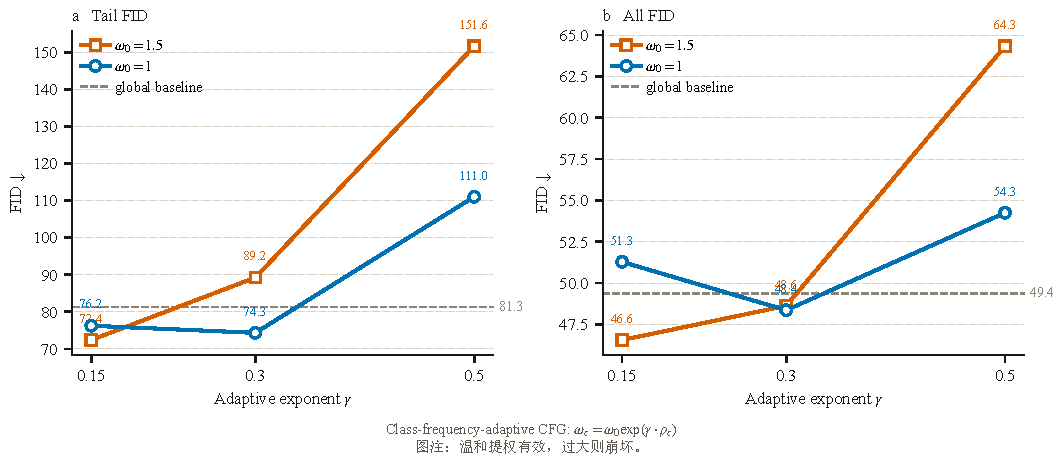
\includegraphics[width=0.48\textwidth]{figures/fig_gamma_sensitivity.pdf}
\caption{Sensitivity of tail and overall FID to the adaptive exponent $\gamma$. Mild exponentiation helps tail classes, but $\gamma=0.50$ degrades FID non-monotonically.}
\label{fig:gamma-sensitivity}
\end{figure}

\section{Conclusion}
A small amount of class-frequency-adaptive CFG can improve tail-class generation without hurting overall quality. The benefit is not monotonic: excessive guidance ($\gamma=0.50$) hurts both tail and overall metrics. The empirical finding is limited to the studied $\rho=100$ benchmark; other datasets and model scales need further validation.

\section*{中文短摘}
本研究对类别不平衡条件下的扩散模型做了自适应分类器自由引导（CFG）的实证审计。以全局 CFG$=1.5$、$\eta=1.0$ 为基线（head/mid/tail/all FID 分别为 $46.654$/$66.215$/$81.279$/$49.367$），按类频率调整引导强度 $\omega(c)=\omega_0\exp(\gamma\rho_c)$。结果显示：温和提权（$\omega_0=1.5,\gamma=0.15$）可同时改善 tail 与整体 FID，分别降至 $72.387$ 与 $46.554$；但 $\gamma$ 过大（如 $0.50$）会导致 tail FID 非单调崩坏（$\omega_0=1.5$ 时达 $151.620$）。全部数字来自 gate\_rho100\_200k.csv 与各 adaptive\_w*\_g*/summary.json，未作编造。本结论仅限于 $\rho=100$、$N=2000$ 的实验设置，未引入 schedule-blend 或 guidance-annealing 等已被 Run001 否定的卖点。

\bibliographystyle{IEEEtran}
\bibliography{refs}

\end{document}
